% REV00 Tue 04 May 2021 13:55:16 WIB
% START Tue 04 May 2021 13:55:16 WIB

\chapter{XXX}

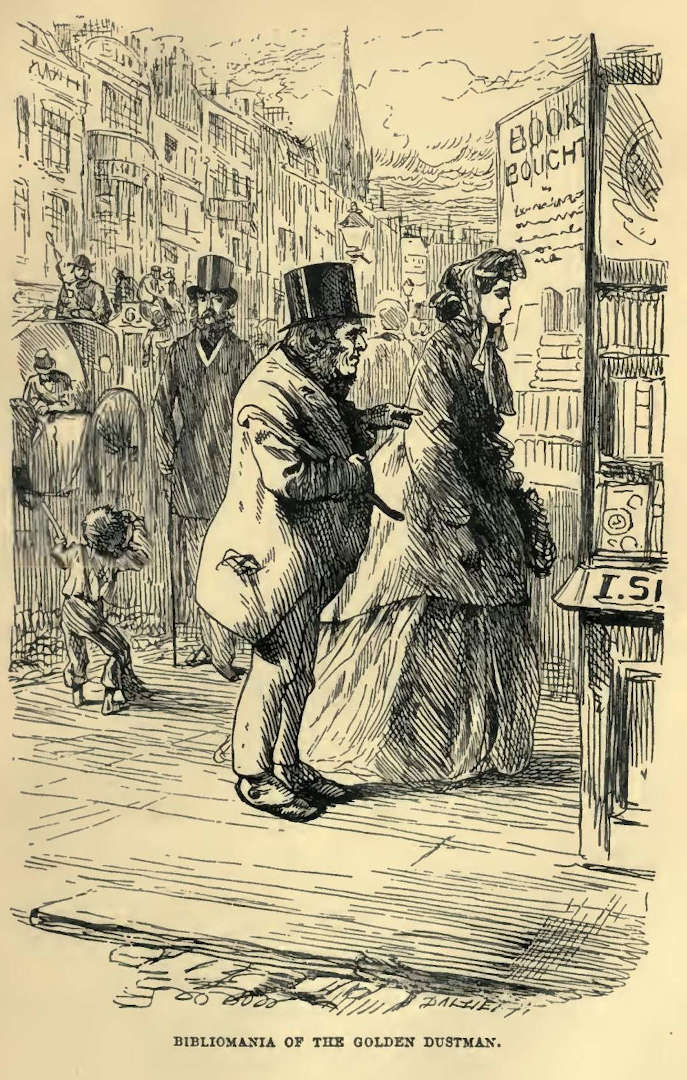
\includegraphics[scale=2.3]{03-05-01}

Chapter 16

THE FEAST OF THE THREE HOBGOBLINS


The City looked unpromising enough, as Bella made her way along its
gritty streets. Most of its money-mills were slackening sail, or had
left off grinding for the day. The master-millers had already departed,
and the journeymen were departing. There was a jaded aspect on
the business lanes and courts, and the very pavements had a weary
appearance, confused by the tread of a million of feet. There must be
hours of night to temper down the day’s distraction of so feverish a
place. As yet the worry of the newly-stopped whirling and grinding on
the part of the money-mills seemed to linger in the air, and the quiet
was more like the prostration of a spent giant than the repose of one
who was renewing his strength.

If Bella thought, as she glanced at the mighty Bank, how agreeable it
would be to have an hour’s gardening there, with a bright copper shovel,
among the money, still she was not in an avaricious vein. Much improved
in that respect, and with certain half-formed images which had little
gold in their composition, dancing before her bright eyes, she arrived
in the drug-flavoured region of Mincing Lane, with the sensation of
having just opened a drawer in a chemist’s shop.

The counting-house of Chicksey, Veneering, and Stobbles was pointed out
by an elderly female accustomed to the care of offices, who dropped upon
Bella out of a public-house, wiping her mouth, and accounted for its
humidity on natural principles well known to the physical sciences, by
explaining that she had looked in at the door to see what o’clock it
was. The counting-house was a wall-eyed ground floor by a dark gateway,
and Bella was considering, as she approached it, could there be any
precedent in the City for her going in and asking for R. Wilfer, when
whom should she see, sitting at one of the windows with the plate-glass
sash raised, but R. Wilfer himself, preparing to take a slight
refection.

On approaching nearer, Bella discerned that the refection had
the appearance of a small cottage-loaf and a pennyworth of milk.
Simultaneously with this discovery on her part, her father discovered
her, and invoked the echoes of Mincing Lane to exclaim ‘My gracious me!’

He then came cherubically flying out without a hat, and embraced her,
and handed her in. ‘For it’s after hours and I am all alone, my dear,’
he explained, ‘and am having--as I sometimes do when they are all
gone--a quiet tea.’

Looking round the office, as if her father were a captive and this his
cell, Bella hugged him and choked him to her heart’s content.

‘I never was so surprised, my dear!’ said her father. ‘I couldn’t
believe my eyes. Upon my life, I thought they had taken to lying! The
idea of your coming down the Lane yourself! Why didn’t you send the
footman down the Lane, my dear?’

‘I have brought no footman with me, Pa.’

‘Oh indeed! But you have brought the elegant turn-out, my love?’

‘No, Pa.’

‘You never can have walked, my dear?’

‘Yes, I have, Pa.’

He looked so very much astonished, that Bella could not make up her mind
to break it to him just yet.

‘The consequence is, Pa, that your lovely woman feels a little faint,
and would very much like to share your tea.’

The cottage loaf and the pennyworth of milk had been set forth on a
sheet of paper on the window-seat. The cherubic pocket-knife, with the
first bit of the loaf still on its point, lay beside them where it had
been hastily thrown down. Bella took the bit off, and put it in her
mouth. ‘My dear child,’ said her father, ‘the idea of your partaking of
such lowly fare! But at least you must have your own loaf and your own
penn’orth. One moment, my dear. The Dairy is just over the way and round
the corner.’

Regardless of Bella’s dissuasions he ran out, and quickly returned with
the new supply. ‘My dear child,’ he said, as he spread it on another
piece of paper before her, ‘the idea of a splendid--!’ and then looked
at her figure, and stopped short.

‘What’s the matter, Pa?’

‘--of a splendid female,’ he resumed more slowly, ‘putting up with
such accommodation as the present!--Is that a new dress you have on, my
dear?’

‘No, Pa, an old one. Don’t you remember it?’

‘Why, I THOUGHT I remembered it, my dear!’

‘You should, for you bought it, Pa.’

‘Yes, I THOUGHT I bought it my dear!’ said the cherub, giving himself a
little shake, as if to rouse his faculties.

‘And have you grown so fickle that you don’t like your own taste, Pa
dear?’

‘Well, my love,’ he returned, swallowing a bit of the cottage loaf with
considerable effort, for it seemed to stick by the way: ‘I should have
thought it was hardly sufficiently splendid for existing circumstances.’

‘And so, Pa,’ said Bella, moving coaxingly to his side instead of
remaining opposite, ‘you sometimes have a quiet tea here all alone? I
am not in the tea’s way, if I draw my arm over your shoulder like this,
Pa?’

‘Yes, my dear, and no, my dear. Yes to the first question, and Certainly
Not to the second. Respecting the quiet tea, my dear, why you see the
occupations of the day are sometimes a little wearing; and if there’s
nothing interposed between the day and your mother, why SHE is sometimes
a little wearing, too.’

‘I know, Pa.’

‘Yes, my dear. So sometimes I put a quiet tea at the window here, with
a little quiet contemplation of the Lane (which comes soothing), between
the day, and domestic--’

‘Bliss,’ suggested Bella, sorrowfully.

‘And domestic Bliss,’ said her father, quite contented to accept the
phrase.

Bella kissed him. ‘And it is in this dark dingy place of captivity,
poor dear, that you pass all the hours of your life when you are not at
home?’

‘Not at home, or not on the road there, or on the road here, my love.
Yes. You see that little desk in the corner?’

‘In the dark corner, furthest both from the light and from the
fireplace? The shabbiest desk of all the desks?’

‘Now, does it really strike you in that point of view, my dear?’ said
her father, surveying it artistically with his head on one side: ‘that’s
mine. That’s called Rumty’s Perch.’

‘Whose Perch?’ asked Bella with great indignation.

‘Rumty’s. You see, being rather high and up two steps they call it a
Perch. And they call ME Rumty.’

‘How dare they!’ exclaimed Bella.

‘They’re playful, Bella my dear; they’re playful. They’re more or less
younger than I am, and they’re playful. What does it matter? It might
be Surly, or Sulky, or fifty disagreeable things that I really shouldn’t
like to be considered. But Rumty! Lor, why not Rumty?’

To inflict a heavy disappointment on this sweet nature, which had been,
through all her caprices, the object of her recognition, love, and
admiration from infancy, Bella felt to be the hardest task of her hard
day. ‘I should have done better,’ she thought, ‘to tell him at first;
I should have done better to tell him just now, when he had some slight
misgiving; he is quite happy again, and I shall make him wretched.’

He was falling back on his loaf and milk, with the pleasantest
composure, and Bella stealing her arm a little closer about him, and at
the same time sticking up his hair with an irresistible propensity
to play with him founded on the habit of her whole life, had prepared
herself to say: ‘Pa dear, don’t be cast down, but I must tell you
something disagreeable!’ when he interrupted her in an unlooked-for
manner.

‘My gracious me!’ he exclaimed, invoking the Mincing Lane echoes as
before. ‘This is very extraordinary!’

‘What is, Pa?’

‘Why here’s Mr Rokesmith now!’

‘No, no, Pa, no,’ cried Bella, greatly flurried. ‘Surely not.’

‘Yes there is! Look here!’

Sooth to say, Mr Rokesmith not only passed the window, but came into the
counting-house. And not only came into the counting-house, but, finding
himself alone there with Bella and her father, rushed at Bella and
caught her in his arms, with the rapturous words ‘My dear, dear girl; my
gallant, generous, disinterested, courageous, noble girl!’ And not only
that even, (which one might have thought astonishment enough for one
dose), but Bella, after hanging her head for a moment, lifted it up and
laid it on his breast, as if that were her head’s chosen and lasting
resting-place!

‘I knew you would come to him, and I followed you,’ said Rokesmith. ‘My
love, my life! You ARE mine?’

To which Bella responded, ‘Yes, I AM yours if you think me worth
taking!’ And after that, seemed to shrink to next to nothing in the
clasp of his arms, partly because it was such a strong one on his part,
and partly because there was such a yielding to it on hers.

The cherub, whose hair would have done for itself under the influence of
this amazing spectacle, what Bella had just now done for it, staggered
back into the window-seat from which he had risen, and surveyed the pair
with his eyes dilated to their utmost.

‘But we must think of dear Pa,’ said Bella; ‘I haven’t told dear Pa; let
us speak to Pa.’ Upon which they turned to do so.

‘I wish first, my dear,’ remarked the cherub faintly, ‘that you’d have
the kindness to sprinkle me with a little milk, for I feel as if I
was--Going.’

In fact, the good little fellow had become alarmingly limp, and his
senses seemed to be rapidly escaping, from the knees upward. Bella
sprinkled him with kisses instead of milk, but gave him a little of that
article to drink; and he gradually revived under her caressing care.

‘We’ll break it to you gently, dearest Pa,’ said Bella.

‘My dear,’ returned the cherub, looking at them both, ‘you broke so much
in the first--Gush, if I may so express myself--that I think I am equal
to a good large breakage now.’

‘Mr Wilfer,’ said John Rokesmith, excitedly and joyfully, ‘Bella takes
me, though I have no fortune, even no present occupation; nothing but
what I can get in the life before us. Bella takes me!’

‘Yes, I should rather have inferred, my dear sir,’ returned the cherub
feebly, ‘that Bella took you, from what I have within these few minutes
remarked.’

‘You don’t know, Pa,’ said Bella, ‘how ill I have used him!’

‘You don’t know, sir,’ said Rokesmith, ‘what a heart she has!’

‘You don’t know, Pa,’ said Bella, ‘what a shocking creature I was
growing, when he saved me from myself!’

‘You don’t know, sir,’ said Rokesmith, ‘what a sacrifice she has made
for me!’

‘My dear Bella,’ replied the cherub, still pathetically scared, ‘and my
dear John Rokesmith, if you will allow me so to call you--’

‘Yes do, Pa, do!’ urged Bella. ‘I allow you, and my will is his law.
Isn’t it--dear John Rokesmith?’

There was an engaging shyness in Bella, coupled with an engaging
tenderness of love and confidence and pride, in thus first calling him
by name, which made it quite excusable in John Rokesmith to do what he
did. What he did was, once more to give her the appearance of vanishing
as aforesaid.

‘I think, my dears,’ observed the cherub, ‘that if you could make it
convenient to sit one on one side of me, and the other on the other, we
should get on rather more consecutively, and make things rather
plainer. John Rokesmith mentioned, a while ago, that he had no present
occupation.’

‘None,’ said Rokesmith.

‘No, Pa, none,’ said Bella.

‘From which I argue,’ proceeded the cherub, ‘that he has left Mr
Boffin?’

‘Yes, Pa. And so--’

‘Stop a bit, my dear. I wish to lead up to it by degrees. And that Mr
Boffin has not treated him well?’

‘Has treated him most shamefully, dear Pa!’ cried Bella with a flashing
face.

‘Of which,’ pursued the cherub, enjoining patience with his hand, ‘a
certain mercenary young person distantly related to myself, could not
approve? Am I leading up to it right?’

‘Could not approve, sweet Pa,’ said Bella, with a tearful laugh and a
joyful kiss.

‘Upon which,’ pursued the cherub, ‘the certain mercenary young person
distantly related to myself, having previously observed and mentioned
to myself that prosperity was spoiling Mr Boffin, felt that she must not
sell her sense of what was right and what was wrong, and what was true
and what was false, and what was just and what was unjust, for any
price that could be paid to her by any one alive? Am I leading up to it
right?’

With another tearful laugh Bella joyfully kissed him again.

‘And therefore--and therefore,’ the cherub went on in a glowing voice,
as Bella’s hand stole gradually up his waistcoat to his neck, ‘this
mercenary young person distantly related to myself, refused the
price, took off the splendid fashions that were part of it, put on the
comparatively poor dress that I had last given her, and trusting to my
supporting her in what was right, came straight to me. Have I led up to
it?’

Bella’s hand was round his neck by this time, and her face was on it.

‘The mercenary young person distantly related to myself,’ said her
good father, ‘did well! The mercenary young person distantly related
to myself, did not trust to me in vain! I admire this mercenary young
person distantly related to myself, more in this dress than if she had
come to me in China silks, Cashmere shawls, and Golconda diamonds. I
love this young person dearly. I say to the man of this young person’s
heart, out of my heart and with all of it, “My blessing on this
engagement betwixt you, and she brings you a good fortune when she
brings you the poverty she has accepted for your sake and the honest
truth’s!”’

The stanch little man’s voice failed him as he gave John Rokesmith his
hand, and he was silent, bending his face low over his daughter. But,
not for long. He soon looked up, saying in a sprightly tone:

‘And now, my dear child, if you think you can entertain John Rokesmith
for a minute and a half, I’ll run over to the Dairy, and fetch HIM a
cottage loaf and a drink of milk, that we may all have tea together.’

It was, as Bella gaily said, like the supper provided for the three
nursery hobgoblins at their house in the forest, without their
thunderous low growlings of the alarming discovery, ‘Somebody’s been
drinking MY milk!’ It was a delicious repast; by far the most delicious
that Bella, or John Rokesmith, or even R. Wilfer had ever made. The
uncongenial oddity of its surroundings, with the two brass knobs of the
iron safe of Chicksey, Veneering, and Stobbles staring from a corner,
like the eyes of some dull dragon, only made it the more delightful.

‘To think,’ said the cherub, looking round the office with unspeakable
enjoyment, ‘that anything of a tender nature should come off here, is
what tickles me. To think that ever I should have seen my Bella folded
in the arms of her future husband, HERE, you know!’

It was not until the cottage loaves and the milk had for some time
disappeared, and the foreshadowings of night were creeping over Mincing
Lane, that the cherub by degrees became a little nervous, and said to
Bella, as he cleared his throat:

‘Hem!--Have you thought at all about your mother, my dear?’

‘Yes, Pa.’

‘And your sister Lavvy, for instance, my dear?’

‘Yes, Pa. I think we had better not enter into particulars at home. I
think it will be quite enough to say that I had a difference with Mr
Boffin, and have left for good.’

‘John Rokesmith being acquainted with your Ma, my love,’ said her
father, after some slight hesitation, ‘I need have no delicacy in
hinting before him that you may perhaps find your Ma a little wearing.’

‘A little, patient Pa?’ said Bella with a tuneful laugh: the tune fuller
for being so loving in its tone.

‘Well! We’ll say, strictly in confidence among ourselves, wearing;
we won’t qualify it,’ the cherub stoutly admitted. ‘And your sister’s
temper is wearing.’

‘I don’t mind, Pa.’

‘And you must prepare yourself you know, my precious,’ said her father,
with much gentleness, ‘for our looking very poor and meagre at home, and
being at the best but very uncomfortable, after Mr Boffin’s house.’

‘I don’t mind, Pa. I could bear much harder trials--for John.’

The closing words were not so softly and blushingly said but that John
heard them, and showed that he heard them by again assisting Bella to
another of those mysterious disappearances.

‘Well!’ said the cherub gaily, and not expressing disapproval, ‘when
you--when you come back from retirement, my love, and reappear on the
surface, I think it will be time to lock up and go.’

If the counting-house of Chicksey, Veneering, and Stobbles had ever been
shut up by three happier people, glad as most people were to shut it up,
they must have been superlatively happy indeed. But first Bella mounted
upon Rumty’s Perch, and said, ‘Show me what you do here all day long,
dear Pa. Do you write like this?’ laying her round cheek upon her plump
left arm, and losing sight of her pen in waves of hair, in a highly
unbusiness-like manner. Though John Rokesmith seemed to like it.

So, the three hobgoblins, having effaced all traces of their feast, and
swept up the crumbs, came out of Mincing Lane to walk to Holloway; and
if two of the hobgoblins didn’t wish the distance twice as long as it
was, the third hobgoblin was much mistaken. Indeed, that modest spirit
deemed himself so much in the way of their deep enjoyment of the
journey, that he apologetically remarked: ‘I think, my dears, I’ll take
the lead on the other side of the road, and seem not to belong to you.’
Which he did, cherubically strewing the path with smiles, in the absence
of flowers.

It was almost ten o’clock when they stopped within view of Wilfer
Castle; and then, the spot being quiet and deserted, Bella began a
series of disappearances which threatened to last all night.

‘I think, John,’ the cherub hinted at last, ‘that if you can spare me
the young person distantly related to myself, I’ll take her in.’

‘I can’t spare her,’ answered John, ‘but I must lend her to you.--My
Darling!’ A word of magic which caused Bella instantly to disappear
again.

‘Now, dearest Pa,’ said Bella, when she became visible, ‘put your hand
in mine, and we’ll run home as fast as ever we can run, and get it over.
Now, Pa. Once!--’

‘My dear,’ the cherub faltered, with something of a craven air, ‘I was
going to observe that if your mother--’

‘You mustn’t hang back, sir, to gain time,’ cried Bella, putting out her
right foot; ‘do you see that, sir? That’s the mark; come up to the mark,
sir. Once! Twice! Three times and away, Pa!’ Off she skimmed, bearing
the cherub along, nor ever stopped, nor suffered him to stop, until she
had pulled at the bell. ‘Now, dear Pa,’ said Bella, taking him by both
ears as if he were a pitcher, and conveying his face to her rosy lips,
‘we are in for it!’

Miss Lavvy came out to open the gate, waited on by that attentive
cavalier and friend of the family, Mr George Sampson. ‘Why, it’s never
Bella!’ exclaimed Miss Lavvy starting back at the sight. And then
bawled, ‘Ma! Here’s Bella!’

This produced, before they could get into the house, Mrs Wilfer. Who,
standing in the portal, received them with ghostly gloom, and all her
other appliances of ceremony.

‘My child is welcome, though unlooked for,’ said she, at the time
presenting her cheek as if it were a cool slate for visitors to enrol
themselves upon. ‘You too, R. W., are welcome, though late. Does the
male domestic of Mrs Boffin hear me there?’ This deep-toned inquiry was
cast forth into the night, for response from the menial in question.

‘There is no one waiting, Ma, dear,’ said Bella.

‘There is no one waiting?’ repeated Mrs Wilfer in majestic accents.

‘No, Ma, dear.’

A dignified shiver pervaded Mrs Wilfer’s shoulders and gloves, as
who should say, ‘An Enigma!’ and then she marched at the head of the
procession to the family keeping-room, where she observed:

‘Unless, R. W.’: who started on being solemnly turned upon: ‘you have
taken the precaution of making some addition to our frugal supper on
your way home, it will prove but a distasteful one to Bella. Cold neck
of mutton and a lettuce can ill compete with the luxuries of Mr Boffin’s
board.’

‘Pray don’t talk like that, Ma dear,’ said Bella; ‘Mr Boffin’s board is
nothing to me.’

But, here Miss Lavinia, who had been intently eyeing Bella’s bonnet,
struck in with ‘Why, Bella!’

‘Yes, Lavvy, I know.’

The Irrepressible lowered her eyes to Bella’s dress, and stooped to look
at it, exclaiming again: ‘Why, Bella!’

‘Yes, Lavvy, I know what I have got on. I was going to tell Ma when you
interrupted. I have left Mr Boffin’s house for good, Ma, and I have come
home again.’

Mrs Wilfer spake no word, but, having glared at her offspring for a
minute or two in an awful silence, retired into her corner of state
backward, and sat down: like a frozen article on sale in a Russian
market.

‘In short, dear Ma,’ said Bella, taking off the depreciated bonnet and
shaking out her hair, ‘I have had a very serious difference with Mr
Boffin on the subject of his treatment of a member of his household, and
it’s a final difference, and there’s an end of all.’

‘And I am bound to tell you, my dear,’ added R. W., submissively, ‘that
Bella has acted in a truly brave spirit, and with a truly right feeling.
And therefore I hope, my dear, you’ll not allow yourself to be greatly
disappointed.’

‘George!’ said Miss Lavvy, in a sepulchral, warning voice, founded on
her mother’s; ‘George Sampson, speak! What did I tell you about those
Boffins?’

Mr Sampson perceiving his frail bark to be labouring among shoals and
breakers, thought it safest not to refer back to any particular thing
that he had been told, lest he should refer back to the wrong thing.
With admirable seamanship he got his bark into deep water by murmuring
‘Yes indeed.’

‘Yes! I told George Sampson, as George Sampson tells you,’ said Miss
Lavvy, ‘that those hateful Boffins would pick a quarrel with Bella, as
soon as her novelty had worn off. Have they done it, or have they not?
Was I right, or was I wrong? And what do you say to us, Bella, of your
Boffins now?’

‘Lavvy and Ma,’ said Bella, ‘I say of Mr and Mrs Boffin what I always
have said; and I always shall say of them what I always have said. But
nothing will induce me to quarrel with any one to-night. I hope you
are not sorry to see me, Ma dear,’ kissing her; ‘and I hope you are not
sorry to see me, Lavvy,’ kissing her too; ‘and as I notice the lettuce
Ma mentioned, on the table, I’ll make the salad.’

Bella playfully setting herself about the task, Mrs Wilfer’s impressive
countenance followed her with glaring eyes, presenting a combination
of the once popular sign of the Saracen’s Head, with a piece of
Dutch clock-work, and suggesting to an imaginative mind that from the
composition of the salad, her daughter might prudently omit the vinegar.
But no word issued from the majestic matron’s lips. And this was more
terrific to her husband (as perhaps she knew) than any flow of eloquence
with which she could have edified the company.

‘Now, Ma dear,’ said Bella in due course, ‘the salad’s ready, and it’s
past supper-time.’

Mrs Wilfer rose, but remained speechless. ‘George!’ said Miss Lavinia
in her voice of warning, ‘Ma’s chair!’ Mr Sampson flew to the excellent
lady’s back, and followed her up close chair in hand, as she stalked
to the banquet. Arrived at the table, she took her rigid seat, after
favouring Mr Sampson with a glare for himself, which caused the young
gentleman to retire to his place in much confusion.

The cherub not presuming to address so tremendous an object, transacted
her supper through the agency of a third person, as ‘Mutton to your Ma,
Bella, my dear’; and ‘Lavvy, I dare say your Ma would take some lettuce
if you were to put it on her plate.’ Mrs Wilfer’s manner of receiving
those viands was marked by petrified absence of mind; in which state,
likewise, she partook of them, occasionally laying down her knife and
fork, as saying within her own spirit, ‘What is this I am doing?’ and
glaring at one or other of the party, as if in indignant search of
information. A magnetic result of such glaring was, that the person
glared at could not by any means successfully pretend to be ignorant of
the fact: so that a bystander, without beholding Mrs Wilfer at all, must
have known at whom she was glaring, by seeing her refracted from the
countenance of the beglared one.

Miss Lavinia was extremely affable to Mr Sampson on this special
occasion, and took the opportunity of informing her sister why.

‘It was not worth troubling you about, Bella, when you were in a sphere
so far removed from your family as to make it a matter in which you
could be expected to take very little interest,’ said Lavinia with a
toss of her chin; ‘but George Sampson is paying his addresses to me.’

Bella was glad to hear it. Mr Sampson became thoughtfully red, and
felt called upon to encircle Miss Lavinia’s waist with his arm; but,
encountering a large pin in the young lady’s belt, scarified a finger,
uttered a sharp exclamation, and attracted the lightning of Mrs Wilfer’s
glare.

‘George is getting on very well,’ said Miss Lavinia which might not have
been supposed at the moment--‘and I dare say we shall be married, one of
these days. I didn’t care to mention it when you were with your Bof--’
here Miss Lavinia checked herself in a bounce, and added more placidly,
‘when you were with Mr and Mrs Boffin; but now I think it sisterly to
name the circumstance.’

‘Thank you, Lavvy dear. I congratulate you.’

‘Thank you, Bella. The truth is, George and I did discuss whether
I should tell you; but I said to George that you wouldn’t be much
interested in so paltry an affair, and that it was far more likely you
would rather detach yourself from us altogether, than have him added to
the rest of us.’

‘That was a mistake, dear Lavvy,’ said Bella.

‘It turns out to be,’ replied Miss Lavinia; ‘but circumstances have
changed, you know, my dear. George is in a new situation, and his
prospects are very good indeed. I shouldn’t have had the courage to tell
you so yesterday, when you would have thought his prospects poor, and
not worth notice; but I feel quite bold tonight.’

‘When did you begin to feel timid, Lavvy?’ inquired Bella, with a smile.

‘I didn’t say that I ever felt timid, Bella,’ replied the Irrepressible.
‘But perhaps I might have said, if I had not been restrained by delicacy
towards a sister’s feelings, that I have for some time felt independent;
too independent, my dear, to subject myself to have my intended match
(you’ll prick yourself again, George) looked down upon. It is not that I
could have blamed you for looking down upon it, when you were looking up
to a rich and great match, Bella; it is only that I was independent.’

Whether the Irrepressible felt slighted by Bella’s declaration that she
would not quarrel, or whether her spitefulness was evoked by Bella’s
return to the sphere of Mr George Sampson’s courtship, or whether it was
a necessary fillip to her spirits that she should come into collision
with somebody on the present occasion,--anyhow she made a dash at her
stately parent now, with the greatest impetuosity.

‘Ma, pray don’t sit staring at me in that intensely aggravating manner!
If you see a black on my nose, tell me so; if you don’t, leave me
alone.’

‘Do you address Me in those words?’ said Mrs Wilfer. ‘Do you presume?’

‘Don’t talk about presuming, Ma, for goodness’ sake. A girl who is old
enough to be engaged, is quite old enough to object to be stared at as
if she was a Clock.’

‘Audacious one!’ said Mrs Wilfer. ‘Your grandmamma, if so addressed by
one of her daughters, at any age, would have insisted on her retiring to
a dark apartment.’

‘My grandmamma,’ returned Lavvy, folding her arms and leaning back
in her chair, ‘wouldn’t have sat staring people out of countenance, I
think.’

‘She would!’ said Mrs Wilfer.

‘Then it’s a pity she didn’t know better,’ said Lavvy. ‘And if my
grandmamma wasn’t in her dotage when she took to insisting on people’s
retiring to dark apartments, she ought to have been. A pretty exhibition
my grandmamma must have made of herself! I wonder whether she ever
insisted on people’s retiring into the ball of St Paul’s; and if she
did, how she got them there!’

‘Silence!’ proclaimed Mrs Wilfer. ‘I command silence!’

‘I have not the slightest intention of being silent, Ma,’ returned
Lavinia coolly, ‘but quite the contrary. I am not going to be eyed as if
I had come from the Boffins, and sit silent under it. I am not going
to have George Sampson eyed as if HE had come from the Boffins, and sit
silent under it. If Pa thinks proper to be eyed as if HE had come from
the Boffins also, well and good. I don’t choose to. And I won’t!’

Lavinia’s engineering having made this crooked opening at Bella, Mrs
Wilfer strode into it.

‘You rebellious spirit! You mutinous child! Tell me this, Lavinia. If
in violation of your mother’s sentiments, you had condescended to allow
yourself to be patronized by the Boffins, and if you had come from those
halls of slavery--’

‘That’s mere nonsense, Ma,’ said Lavinia.

‘How!’ exclaimed Mrs Wilfer, with sublime severity.

‘Halls of slavery, Ma, is mere stuff and nonsense,’ returned the unmoved
Irrepressible.

‘I say, presumptuous child, if you had come from the neighbourhood of
Portland Place, bending under the yoke of patronage and attended by its
domestics in glittering garb to visit me, do you think my deep-seated
feelings could have been expressed in looks?’

‘All I think about it, is,’ returned Lavinia, ‘that I should wish them
expressed to the right person.’

‘And if,’ pursued her mother, ‘if making light of my warnings that the
face of Mrs Boffin alone was a face teeming with evil, you had clung to
Mrs Boffin instead of to me, and had after all come home rejected by Mrs
Boffin, trampled under foot by Mrs Boffin, and cast out by Mrs Boffin,
do you think my feelings could have been expressed in looks?’

Lavinia was about replying to her honoured parent that she might as well
have dispensed with her looks altogether then, when Bella rose and said,
‘Good night, dear Ma. I have had a tiring day, and I’ll go to bed.’ This
broke up the agreeable party. Mr George Sampson shortly afterwards took
his leave, accompanied by Miss Lavinia with a candle as far as the hall,
and without a candle as far as the garden gate; Mrs Wilfer, washing her
hands of the Boffins, went to bed after the manner of Lady Macbeth; and
R. W. was left alone among the dilapidations of the supper table, in a
melancholy attitude.

But, a light footstep roused him from his meditations, and it was
Bella’s. Her pretty hair was hanging all about her, and she had tripped
down softly, brush in hand, and barefoot, to say good-night to him.

‘My dear, you most unquestionably ARE a lovely woman,’ said the cherub,
taking up a tress in his hand.

‘Look here, sir,’ said Bella; ‘when your lovely woman marries, you shall
have that piece if you like, and she’ll make you a chain of it. Would
you prize that remembrance of the dear creature?’

‘Yes, my precious.’

‘Then you shall have it if you’re good, sir. I am very, very sorry,
dearest Pa, to have brought home all this trouble.’

‘My pet,’ returned her father, in the simplest good faith, ‘don’t make
yourself uneasy about that. It really is not worth mentioning, because
things at home would have taken pretty much the same turn any way. If
your mother and sister don’t find one subject to get at times a little
wearing on, they find another. We’re never out of a wearing subject,
my dear, I assure you. I am afraid you find your old room with Lavvy,
dreadfully inconvenient, Bella?’

‘No I don’t, Pa; I don’t mind. Why don’t I mind, do you think, Pa?’

‘Well, my child, you used to complain of it when it wasn’t such a
contrast as it must be now. Upon my word, I can only answer, because you
are so much improved.’

‘No, Pa. Because I am so thankful and so happy!’

Here she choked him until her long hair made him sneeze, and then she
laughed until she made him laugh, and then she choked him again that
they might not be overheard.

‘Listen, sir,’ said Bella. ‘Your lovely woman was told her fortune
to night on her way home. It won’t be a large fortune, because if the
lovely woman’s Intended gets a certain appointment that he hopes to get
soon, she will marry on a hundred and fifty pounds a year. But that’s at
first, and even if it should never be more, the lovely woman will make
it quite enough. But that’s not all, sir. In the fortune there’s a
certain fair man--a little man, the fortune-teller said--who, it seems,
will always find himself near the lovely woman, and will always have
kept, expressly for him, such a peaceful corner in the lovely woman’s
little house as never was. Tell me the name of that man, sir.’

‘Is he a Knave in the pack of cards?’ inquired the cherub, with a
twinkle in his eyes.

‘Yes!’ cried Bella, in high glee, choking him again. ‘He’s the Knave of
Wilfers! Dear Pa, the lovely woman means to look forward to this fortune
that has been told for her, so delightfully, and to cause it to make her
a much better lovely woman than she ever has been yet. What the little
fair man is expected to do, sir, is to look forward to it also, by
saying to himself when he is in danger of being over-worried, “I see
land at last!”

‘I see land at last!’ repeated her father.

‘There’s a dear Knave of Wilfers!’ exclaimed Bella; then putting out her
small white bare foot, ‘That’s the mark, sir. Come to the mark. Put your
boot against it. We keep to it together, mind! Now, sir, you may kiss
the lovely woman before she runs away, so thankful and so happy. O yes,
fair little man, so thankful and so happy!’



